\documentclass[../../manuale-manutentore.tex]{subfiles}

\begin{document}
\subsection{Mobile app}%
\label{sub:mobile_app}

Tutte le classi definite per l'applicazione mobile sono raccolte nel package \java{tech.gruppone.stalker.app}, i cui subpackage sono organizzati come indicato in figura §\ref{fig:app/diagramma_package}
\begin{figure}[h]
  \centering
  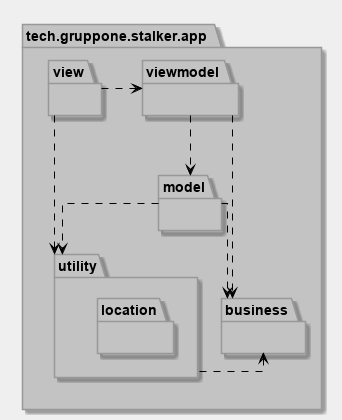
\includegraphics[width=6cm]{app-package-diagram.png}
  \caption{Diagramma dei package per l'applicazione mobile}
~~\label{fig:app/diagramma_package}
\end{figure}

\subsubsection{MVVM}%
\label{subs:mvvm}

Per la mobile app abbiamo scelto il pattern Model-View-ViewModel, in quanto è supportato nativamente dalle librerie di Android e si integra perfettamente con il sistema di lifetime del framework. Per ogni schermata \textit{X} visualizzata dall'utente, ad esempio la schermata di \textit{Login}, sono individuate:
\begin{itemize}
  \item Una classe \java{XActivity} derivata da \java{androidx.appcompat.app.AppCompActivity}, corrispondente alla View, a cui è associato un layout \linebreak[1]\texttt{activity\_x.xml} scritto in XML\@.
  \item Se necessario, una classe \java{XViewModel} derivata da \java{androidx.lifecycle.ViewModel} corrispondente al ViewModel.
  \item Se necessario, una classe \java{XModel} derivata da \java{java.lang.Object} corrispondente al Model.
\end{itemize}

GruppOne raccoglie le classi \java{XActivity}, \java{XViewModel} e \java{XModel} rispettivamente nei subpackage \java{view}, \java{viewmodel} e \java{model}.
Le tre classi formano la gerarchia mostrata in figura §\ref{fig:app/diagramma_classi_mvvm}.
Mentre \java{XViewModel} può semplicemente istanziare \java{Model}, \java{XActivity} deve ricevere un'istanza di \java{XViewModel} da un \java{androidx.lifecycle.ViewModelProvider} attraverso il metodo \java{get(Class<T>)}, a causa del lifetime system.
Ogni volta che un oggetto associato alla stessa schermata, e quindi istanza della stessa classe \java{XActivity}, viene costruito, ad esempio dopo che lo schermo è stato ruotato, il \java{ViewModelProvider} gli restituisce la stessa istanza della classe \java{XViewModel}.
Il modo più comune di ottenere l'istanza di \java{XViewModel}, a meno degli opportuni import, è:

\begin{minted}{java}
class XActivity extends AppCompActivity {
  ...
  private XViewModel viewModel;

  @Override
  protected void onCreate(@Nullable Bundle savedInstanceState) {
    ...
    viewModel = new ViewModelProvider(this).get(XViewModel.class);
    ...
  }
  ...
}
\end{minted}

Siccome i permessi di geolocalizzazione sono necessari al corretto funzionamento dell'applicazione, essa verifica ogni volta che viene aperta o riportata in primo piano che non siano stati revocati.
Per questo abbiamo scelto di utilizzare un decorator pattern, quindi forniamo la classe \java{utility.StalkerActivity} come classe derivata da \java{androidx.appcompat.app.AppCompatActivity} per eseguire automaticamente questa verifica.

\begin{figure}[h]
  \centering
  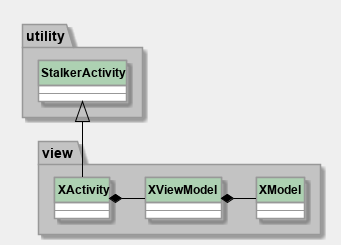
\includegraphics{app-mvvm.png}
  \caption{Diagramma delle classi per MVVM}
~~\label{fig:app/diagramma_classi_mvvm}
\end{figure}

Per quanto riguarda l'autenticazione, e quindi le schermate di \textit{Login} e \textit{Signup}, il viewmodel ha la responsabilità di produrre un hash della password, mentre il model ha la responsabilità di definire il metodo callback che viene invocato quando il server risponde alla richiesta.

\subsubsection{RecyclerView}%
\label{subs:recyclerview}

La schermata principale presenta la lista di organizzazioni a cui l'utente può connettersi, e per questo deve aggiornarsi dinamicamente quando l'applicazione riceve dal server una nuova lista.
A questo scopo abbiamo scelto di utilizzare \java{androidx.recyclerview.widget.RecyclerView}, componente grafica che astrae il confronto fra la lista nuova e quella attuale, richiedendo un minimo quantitativo di codice per specificare come confrontare gli elementi uno ad uno.
Questo deve essere fornito nella forma di un'istanza di una classe derivata da \java{androidx.recyclerview.widget.ListAdapter}, una classe generica con due parametri di tipo.
A questo scopo, GruppOne ha definito la classe \java{utility.OrganizationListAdapter}.
Per l'estensione di \java{ListAdapter} il primo parametro di tipo deve essere sostituito con il tipo degli oggetti nella lista, nel nostro caso \java{business.Organization} (§\ref{subs:logica_di_business}), il secondo con una classe derivata da \java{RecyclerView.ViewHolder}.
Quest'ultima rappresenta un elemento della lista e racchiude metadati sulla sua posizione; ciascun \java{ListAdapter} istanzia e modifica i \java{ViewHolder} a propria necessità per aggiornare la \java{Recyclerview}, quindi essi sono da considerarsi come semplici frammenti della funzionalità del \java{ListAdapter} stesso.
Di conseguenza, la nostra estensione di \java{ViewHolder}, \java{OrgViewHolder}, è innestata nella classe \java{OrganizationListAdapter}. Ogni estensione di \java{ViewHolder} deve essere associata ad un layout XML che descriva la grafica del rispettivo elemento nella lista.\par

Ogni estensione di \java{ListAdapter} deve fornire al costruttore della superclasse un'istanza di \linebreak\java{androidx.recyclerview.widget.DiffUtil.ItemCallback} che definisca metodi per confrontare un elemento della lista nuova con il corrispondente nella lista già presente e verificare se coincidono oppure se non coincidono ma sono comunque equivalenti. Inoltre deve fornire override per i metodi:
\begin{itemize}
  \item\java{public OrgViewHolder onCreateViewHolder(ViewGroup parent, int viewType)}, che deve costruire un \java{ViewHolder} appropriato al contesto grafico, dato da \java{parent}, e della tipologia indicata da \java{viewType}.
  \item\java{public void onBindViewHolder(OrgViewHolder holder, int position)}, che deve eseguire tutte le operazioni necessarie affinché \java{holder} rappresenti correttamente l'elemento in lista alla posizione \java{position}.
  \item\java{public int getItemViewType(int position)}, che deve ritornare la tipologia di \java{ViewHolder} associata alla posizione  \java{position}. In particolare, questo metodo è utile per differenziare ad esempio gli elementi pari dai dispari, e generalmente ritorna una delle costanti definite in \java{R.layout} corrispondenti ai layout associati alle estensioni di \java{ViewHolder}.
\end{itemize}

Le estensioni di \java{ViewHolder} non hanno requisiti rigidi, ma preferibilmente dovrebbero prevedere una cache di riferimenti ad elementi grafici di cui fanno uso, per limitare il numero di chiamate a \java{findViewById(int)}, le quali potrebbero rallentare l'applicazione.

\paragraph{Integrazione con MVVM}%
\label{par:integrazione_con_mvvm}

Il \java{ListAdapter} riceve la nuova lista, con la quale aggiornare la \java{RecyclerView}, attraverso il metodo \java{submitList(List<T>)}.
La lista di organizzazioni viene aggiornata attraverso una richiesta HTTP al server (§\ref{subs:richieste_http}), la quale viene gestita in modo asincrono.
Di conseguenza, come esposto più nei dettagli in §\ref{subs:logica_di_business}, la lista viene mantenuta in un oggetto \java{androidx.lifecycle.MutableLiveData<List<Organization>>}, il quale permette l'implementazione di un observer pattern.
Per mantenere la separazione delle responsabilità, la \java{MainPageActivity} riceve una reference al \java{MutableLiveData} dalla propria istanza di \java{MainPageViewModel}, che a sua volta la riceve dalla propria istanza di \java{MainPageModel}, il quale la ottiene dal \java{CurrentSessionSingleton} che ne ha la ownership.

\begin{figure}[h]
  \centering
  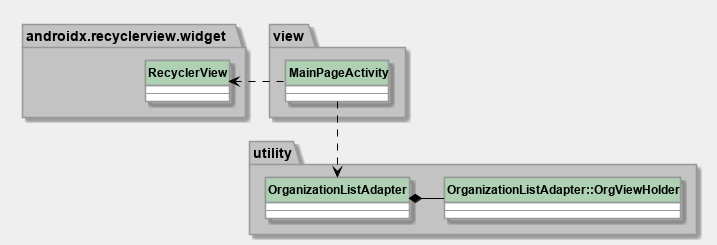
\includegraphics[width=6cm]{app-recyclerview.png}
  \caption{Diagramma delle classi per \java{RecyclerView}}
~~\label{fig:app/diagramma_classi_recyclerview}
\end{figure}

\subsubsection{Classe App}%
\label{subs:classe_app}

In alcune occasioni, ad esempio al momento della creazione della \java{RequestQueue} nel \java{WebSingleton} (§\ref{subs:richieste_http}), è necessario avere accesso al contesto dell'applicazione, rappresentato da un'istanza di \java{android.content.Context}.
Generalmente questo oggetto, condiviso da tutta l'applicazione, si ottiene invocando il metodo \java{getApplicationContext()} su una qualunque istanza di \java{Context} associata ad un'activity.
Per evitare di introdurre dipendenze circolari abbiamo scelto di definire la classe \java{utility.App}, derivata da \java{android.app.Application}, responsabile di mantenere lo stato globale dell'applicazione.
\java{App} ha un metodo aggiuntivo \java{getAppContext()} che espone direttamente il contesto dell'applicazione.

\subsubsection{Richieste HTTP}%
\label{subs:richieste_http}

Per le richieste HTTP abbiamo scelto la libreria \textit{Volley}, consigliata dalle guide ufficiali di Android, perché permette la loro esecuzione asincrona ed efficiente, senza la difficoltà associata alla gestione di un sistema di worker thread.
Le richieste vengono inserite in una struttura a coda gestita da un'istanza di \java{com.android.volley.RequestQueue}, la quale mantiene anche una cache.
Per questo motivo, l'efficienza della libreria migliora se tutte le richieste che l'app effettua sono convogliate nella stessa coda, quindi le guide suggeriscono di astrarre ulteriormente la funzionalità attraverso un singleton.
La classe \java{utility.WebSingleton} espone metodi per eseguire specifiche richieste HTTP al server di Stalker, come \java{login()} o \java{signup()}, ed il metodo \java{addToRequestQueue()} per effettuare una richiesta generica.

\paragraph{Autenticazione}%
\label{par:autenticazione}

Le richieste che richiedono l'autenticazione devono contenere un header \texttt{Authorization} contenente un JWT valido come valore.
La classe \java{utility.AuthenticatedRequest} aggiunge automaticamente questo header, utilizzando il decorator pattern.

\subsubsection{Gestione della posizione}%
\label{subs:gestione_della_posizione}

\subsubsection{Logica di business}%
\label{subs:logica_di_business}

\end{document}
